% F23 Training curves of the two students (30 epochs: job 3614191; 60 epochs: job 3623342). Added 6 Nov.
% Images: results/experiments/exp9_kd_temperature/loss_curves/<RUN>_loss_curves.png from
% scripts/analysis/plot_loss_curves.py (source: the runs' tensorboard events), copied to figures/img/.
% Numbers: data/CLUSTER_ANSWERS.md "6 Nov: loss curves" (slopes over the last 20% of the epochs) -> numbers_nov.tex.
% Plot readings (visible in the images): holdout PVE rises from epoch 5 to 10 (copied heads unfrozen after epoch 5,
% CA "STUDENT DONE"); the training loss drops after each LR halving (every 12 epochs in e30, 24 in e60; exp9 header).
% TODO: the legend draws "train rotmat" and "train kd_out" with the same dash style; replace both PNGs with the fixed
% re-render of plot_loss_curves.py when it arrives (same file names).
\begin{figure}[!p]
\centering
\begin{subfigure}[t]{\linewidth}\centering
  \IfFileExists{figures/img/F23_student_loss_curves_e30.png}{%
    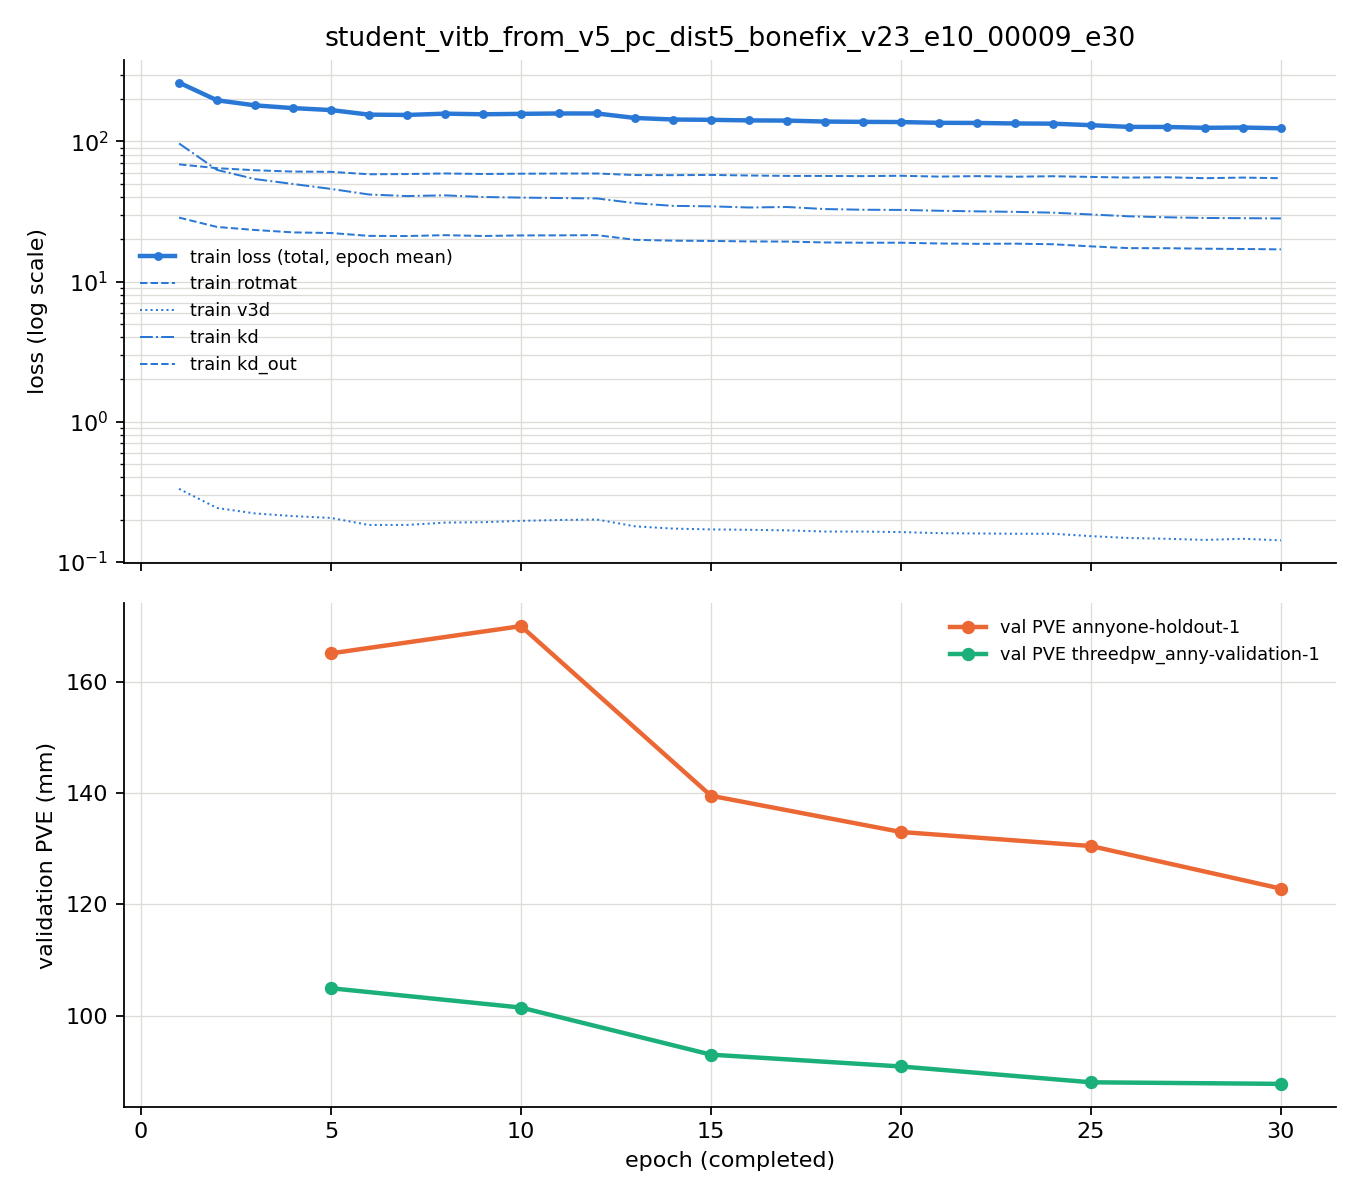
\includegraphics[width=0.62\linewidth]{F23_student_loss_curves_e30.png}}{\fbox{\TODO{F23 e30 image missing}}}
  \caption{Student, \StudentEpochs{} epochs (reported)}\label{fig:loss-curves-e30}
\end{subfigure}

\medskip
\begin{subfigure}[t]{\linewidth}\centering
  \IfFileExists{figures/img/F23_student_loss_curves_e60.png}{%
    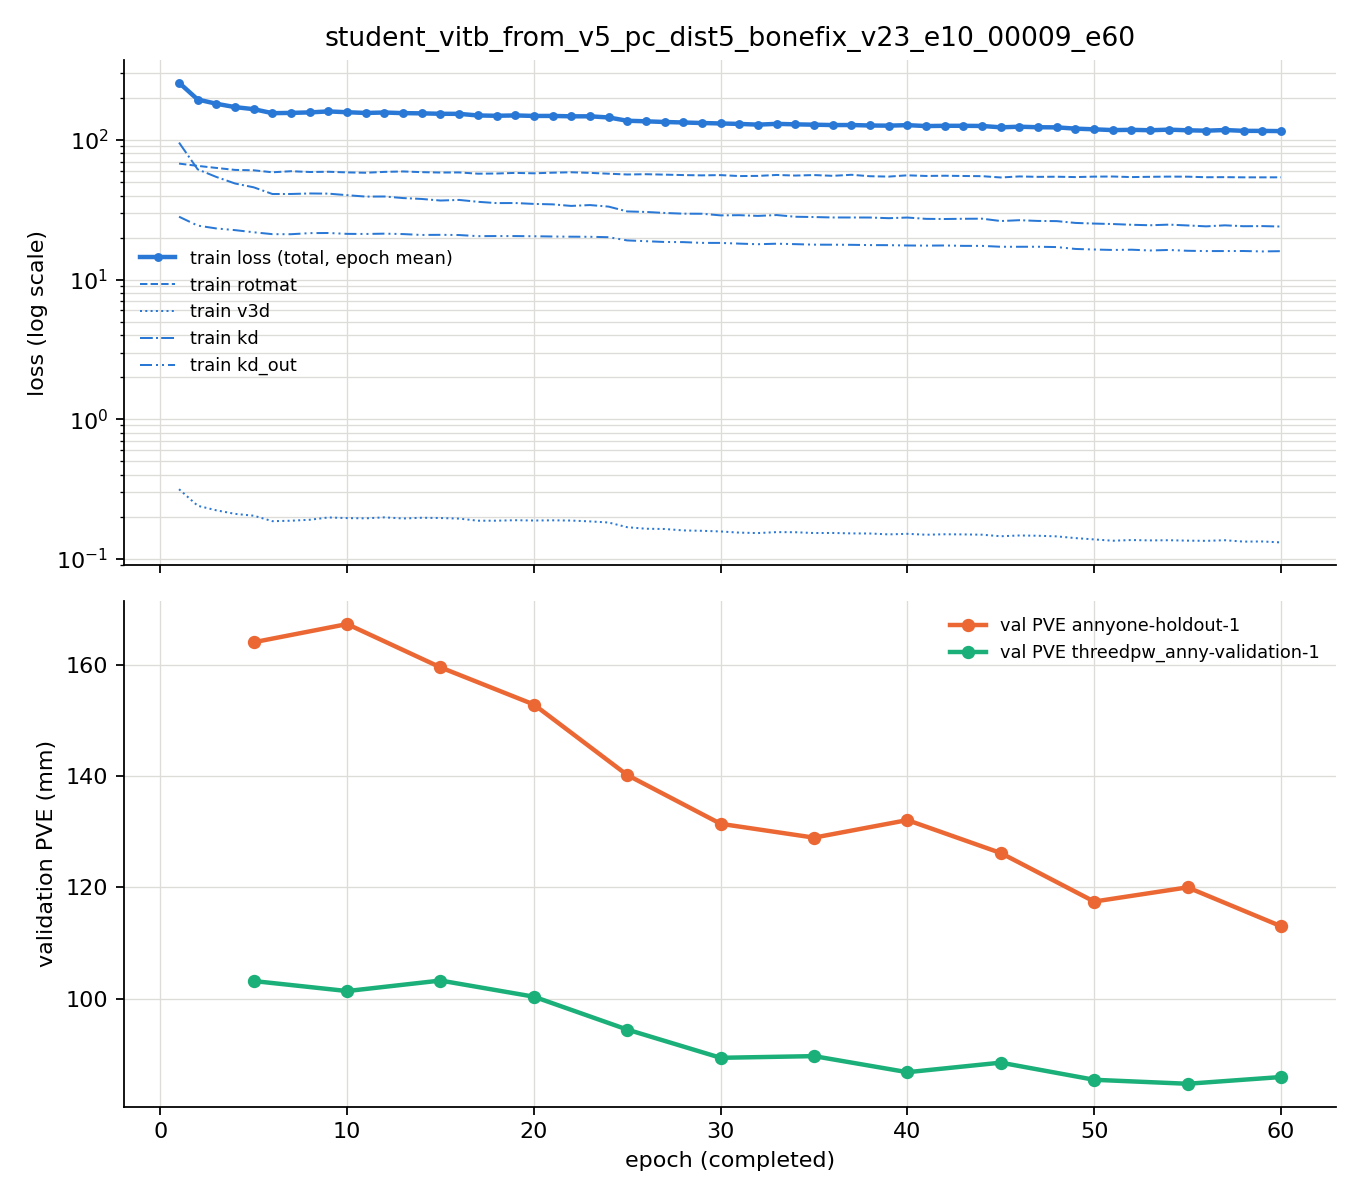
\includegraphics[width=0.62\linewidth]{F23_student_loss_curves_e60.png}}{\fbox{\TODO{F23 e60 image missing}}}
  \caption{Student, \StudentSixtyEpochs{} epochs}\label{fig:loss-curves-e60}
\end{subfigure}
\caption[Training curves of the 30- and 60-epoch students]{Training curves of the Student. Top of each panel: the
training loss per epoch, total and its terms (log scale; the two dashed lines are the rotation term and the output
distillation term, which the legend does not tell apart). Bottom: the validation PVE measured during training every
\LossEvalEvery{} epochs on the AnnyOne holdout and on \LossValImages{} 3DPW-validation images. These runs were
trained before a validation loss was logged, so the validation PVE stands in for it. Over the last 20\,\% of the
epochs (\LossThirtyWindow{} and \LossSixtyWindow) the training loss still falls (\LossThirtyTrainSlope{} and
\LossSixtyTrainSlope\,\% per epoch) and so does the holdout PVE (\LossThirtyHoldSlope{} and
\LossSixtyHoldSlope\,\% per epoch, ending at \LossThirtyHoldLast{} and \LossSixtyHoldLast\,mm), while the 3DPW
validation PVE is flat (\LossThirtyValSlope{} and \LossSixtyValSlope\,\% per epoch, ending at \LossThirtyValLast{} and
\LossSixtyValLast\,mm). The holdout PVE rises between epochs 5 and 10, after the copied heads are unfrozen, and the
large drops follow the learning-rate halvings (every \LossLRHalfThirty{} and \LossLRHalfSixty{} epochs).}
\label{fig:loss-curves}
\label{fig:student-curves}% replaces F19 (in-training curves of the 30-epoch Student)
\end{figure}
